\documentclass[]{IEEEtran}
% some very useful LaTeX packages include:
%\usepackage{cite}      
\usepackage{graphicx}   
\usepackage{subfigure} 
\usepackage{url}       
\usepackage{amsmath}    
\usepackage{caption2}
% Your document starts here!
\begin{document}

% Define document title and author
	\title{Weekly Report}
	\author{Adviser: Prof. Yang Wen \\Student: Cheng Wensheng\\ Period: 2018.6.10-6.17
	}
	\markboth{Visual Information Processing Group}{}
	\maketitle

% Write abstract here
\begin{abstract}
	This week I mainly put my effort on treating Prof. Marcello and reading a paper about using DNN in building extraction of SAR image. 
\end{abstract}

% Each section begins with a \section{title} command
\section{Paper reading}
	% \PARstart{}{} creates a tall first letter for this first paragraph
	\PARstart{T}{he} purpose of this study is to develop a universal classification scheme for most of SAR imagery classification tasks. The well-trained DNN model is used to extract building
	areas from SAR imagery. Extensive validations on different sensors including both
	spaceborne and airborne SAR sensors have been used to verify the accuracy and
	efficiency of the proposed scheme.


	In this study, a DNN-based scheme for SAR imaging classification is introduced. The
	focus of this study is to detect building areas using SAR imagery. Efficient FDN and CNN
	models are trained using advanced deep learning techniques. The proposed method
	allows researchers with limited SAR knowledge to develop their application in a short
	time, without considering the characteristics of SAR sensor. The developed classification
	method is employed to classify SAR imagery obtained by different SAR sensors into
	building and non-building areas based on the FDN and CNN models. The study results
	confirm the high efficiency and accuracy of the proposed classification scheme. 
	
	Fig.~\ref{fig:fw} is the Convolutional neural network (CNN) architecture. Fig.~\ref{fig:rt} is the classification result based on FDN and CNN.
	

% Main Part

\newpage
\begin{figure}[!hbt]
%		 Center the figure.
		\vspace{1.7cm}
%		\hspace{50cm}
		\begin{center}
			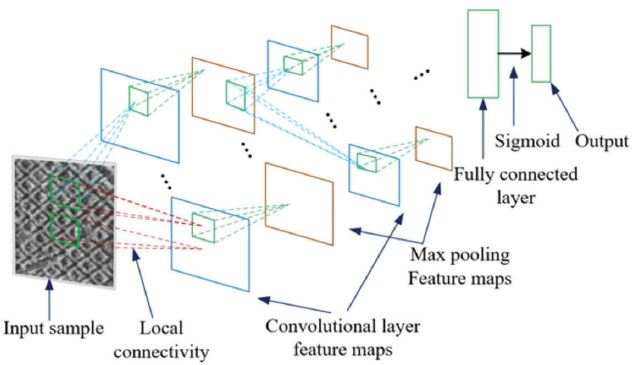
\includegraphics[width=\columnwidth]{fw}
				%		 Create a subtitle for the figure.
			\caption{Convolutional neural network (CNN) architecture}
			\label{fig:fw}
		    \hspace{0.5cm}
			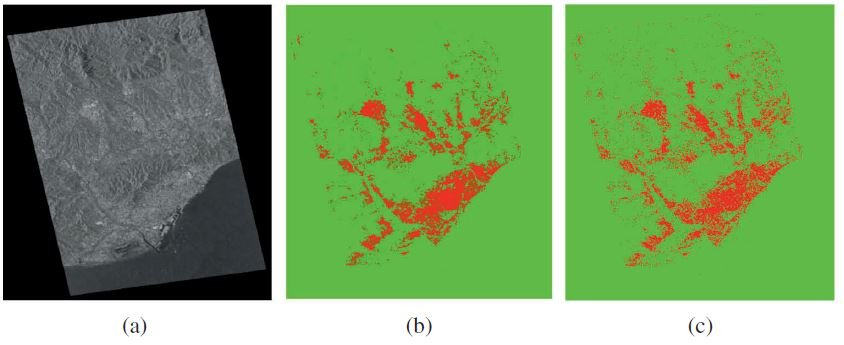
\includegraphics[width=\columnwidth]{rt}
				%Create a subtitle for the figure.
			\caption{Classification result}
			\label{fig:rt}
		\end{center}
	\end{figure}

% Now we need a bibliography:
%\begin{thebibliography}{5}
%
%	%Each item starts with a \bibitem{reference} command and the details thereafter.
%	\bibitem{HOP96} % Transaction paper
%	J.~Hagenauer, E.~Offer, and L.~Papke. Iterative decoding of binary block
%	and convolutional codes. {\em IEEE Trans. Inform. Theory},
%	vol.~42, no.~2, pp.~429–-445, Mar. 1996.
%
%	\bibitem{MJH06} % Conference paper
%	T.~Mayer, H.~Jenkac, and J.~Hagenauer. Turbo base-station cooperation for intercell interference cancellation. {\em IEEE Int. Conf. Commun. (ICC)}, Istanbul, Turkey, pp.~356--361, June 2006.
%
%	\bibitem{Proakis} % Book
%	J.~G.~Proakis. {\em Digital Communications}. McGraw-Hill Book Co.,
%	New York, USA, 3rd edition, 1995.
%
%	\bibitem{talk} % Web document
%	F.~R.~Kschischang. Giving a talk: Guidelines for the Preparation and Presentation of Technical Seminars.
%	\url{http://www.comm.toronto.edu/frank/guide/guide.pdf}.
%
%	\bibitem{5}
%	IEEE Transactions \LaTeX and Microsoft Word Style Files.
%	\url{http://www.ieee.org/web/publications/authors/transjnl/index.html}
%
%\end{thebibliography}

% Your document ends here!
\end{document}